\chapter{VRPTW via AI}
In this chapter, we will review the current end-to-end \gls{ai} methods for solving \gls{vrp} and propose our extension for solving \gls{vrptw}.

Machine learning and artificial intelligence have been replacing many hand-engineered algorithms and providing state-of-the-art results. In recent years, reinforcement learning \ref{rl} and advances in attention models \ref{attention} has shown great promise to disrupt the field of heuristics algorithms \cite{rl-constraint-opt, attention-route, dpdp}. Heuristics algorithms \cite{heuristics-algo} are incomplete methods that can compute solutions efficiently, but are not able to prove the optimality of a solution. Most of the business challenges do not require the most optimal exact solution \cite{excat-algo} but focus on approximation of the optimal solution in a reasonable time.

\section{Related Work}
TODO

\section{Solution}
The end-to-end \gls{ai} method pro solving \gls{vrptw} is extension of the work done by Kool et al. \cite{attention-route}. 

Let us describe the high-level concept behind the method. Consider we have a model as blackbox which takes \gls{vrptw} instance as an input and outputs probabilities for all the \gls{vrptw} nodes. The probability represents which node should be visited next and by following to the most probable node we get a partial solution which will be considered by the blackbox. We iterate this process until all nodes have been visited and we acquire a feasible plan as shown on Figure \ref{fig:attention-route-diagram}.

    \begin{figure}[ht]
        \centering
        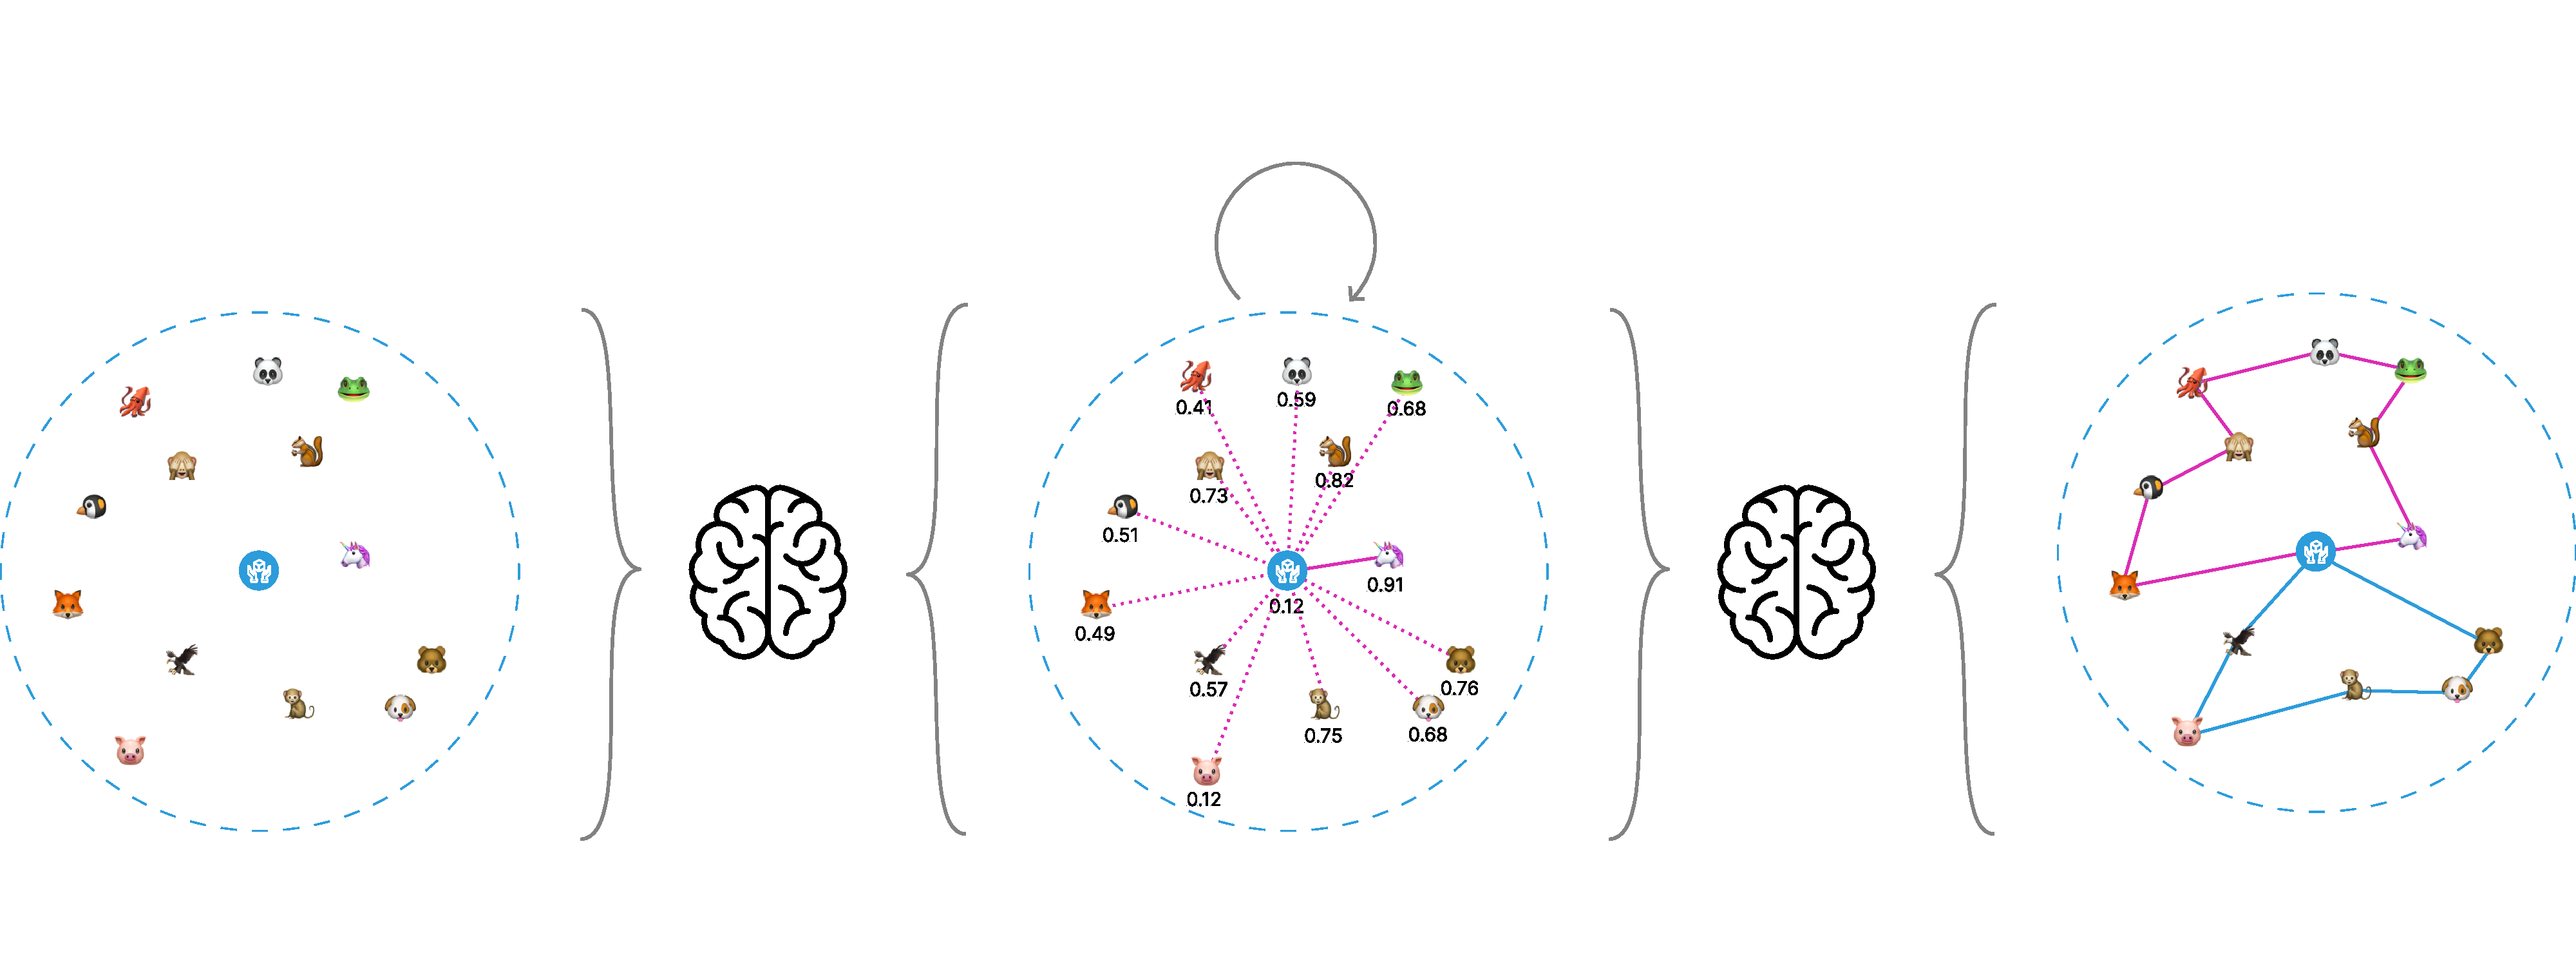
\includegraphics[width=1.0\textwidth]{resources/vrptw-ai/attention-route-diagram.png}
        \caption{High-level concept behind the method our solution}
        \label{fig:attention-route-diagram}
    \end{figure}

    \subsection{Model Architecture}
    The model architucture \cite{attention-route} is advacments of attention mechansims, transformers and graph attention netwoek.
    
    The \gls{vrptw} instance input is consited from
    \begin{itemize}
        \item $X = {x_1, \cdots, x_n})$
        \item $x_0$
        \item $D = {d_1, \cdots, d_n})$
        \item $T = {(e_0, l_0), \cdots, (e_0, l_0)})$
    \end{itemize}
    
    The output
    \begin{itemize}
        \item $\pi = {\pi_1, \cdots, \pi_T} \in {x_0, \cdots, x_n})$ T is longer bacseu of depots
    \end{itemize}
    
    \subsubsection{Encoder}
    
    \subsubsection{Decoder}
        
    \subsection{Reinforcement Learning}
        
    \subsection{Integrating Distance Matrix}
    Multidimensional scaling
